\documentclass[12pt, twoside]{article}
\usepackage[letterpaper, margin=1in, headsep=0.5in]{geometry}
\usepackage[english]{babel}
\usepackage[utf8]{inputenc}
\usepackage{amsmath}
\usepackage{amsfonts}
\usepackage{amssymb}
\usepackage{tikz}
%\usetikzlibrary{quotes, angles}

\usepackage{graphicx}
\usepackage{enumitem}
\usepackage{multicol}

\usepackage{fancyhdr}
\pagestyle{fancy}
\fancyhf{}
\renewcommand{\headrulewidth}{0pt} % disable the underline of the header

\fancyhead[RE]{\thepage}
\fancyhead[RO]{\thepage \\ Name: \hspace{3cm}}
\fancyhead[L]{BECA / Dr. Huson / Geometry\\* 8 December 2019}

\begin{document}
\subsubsection*{6.8 Do Now: Euclid's Garden, mapping angles to slope}
  \begin{enumerate}

    \item Below, right $\triangle ABC$ is shown in standard position with $A(0, 0)$, $B(8, 6)$, and $C(8,0)$.\\[0.25cm]
     Measure the lengths of the sides of the triangle in centimeters and mark them on the diagram.
    \begin{center}
      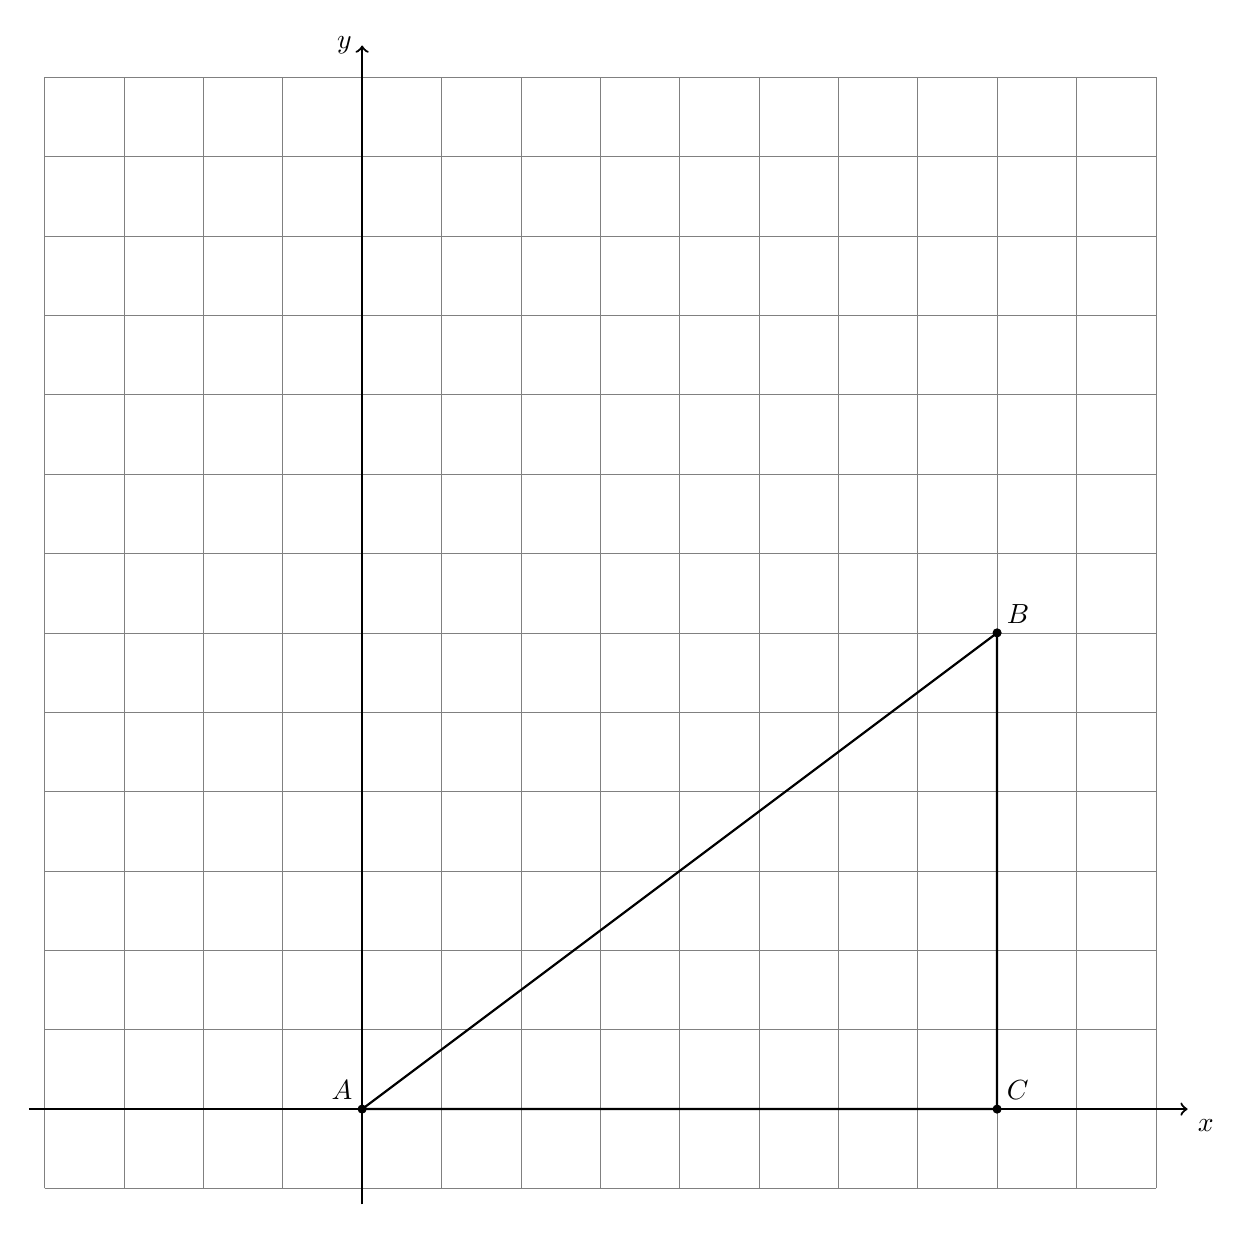
\begin{tikzpicture}[scale=1.008]
        \draw [help lines] (-4,-1) grid (10,13);
        \draw [thick, ->] (-4.2,0) -- (10.4,0) node [below right] {$x$};
        \draw [thick, ->] (0,-1.2)--(0,13.4) node [left] {$y$};
        \draw [thick, -] (0,0)--(8, 6)--(8, 0)--cycle;
        \draw [fill] (0, 0) circle[radius = 0.05] node[above left]{$A$};
        \draw [fill] (8, 6) circle[radius = 0.05] node[above right]{$B$};
        \draw [fill] (8, 0) circle[radius = 0.05] node[above right]{$C$};
      \end{tikzpicture}
    \end{center}
      \vspace{1cm}
    \begin{enumerate}
      \item Mark the vertex of another right triangle in standard position, $D(5,12)$.
      \item Mark the point $E$ on the $x$-axis such that $\overline{AE} \perp \overline{DE}$.
      \item Measure and mark the dimensions of $\triangle ADE$ on the graph.
    \end{enumerate}

\newpage 
  \item Complete the t-chart for $x= -3,-2,-1,0,1,2,3$, then graph and label the function on the grid below, labeling the vertex on the graph as an ordered pair.\\[0.25cm]
  Use pencil for graphs. Draw parabolas as smooth curves.

  \[f(x) = x^2\]

    \begin{center} %4 quadrant regents grid w T-Chart
      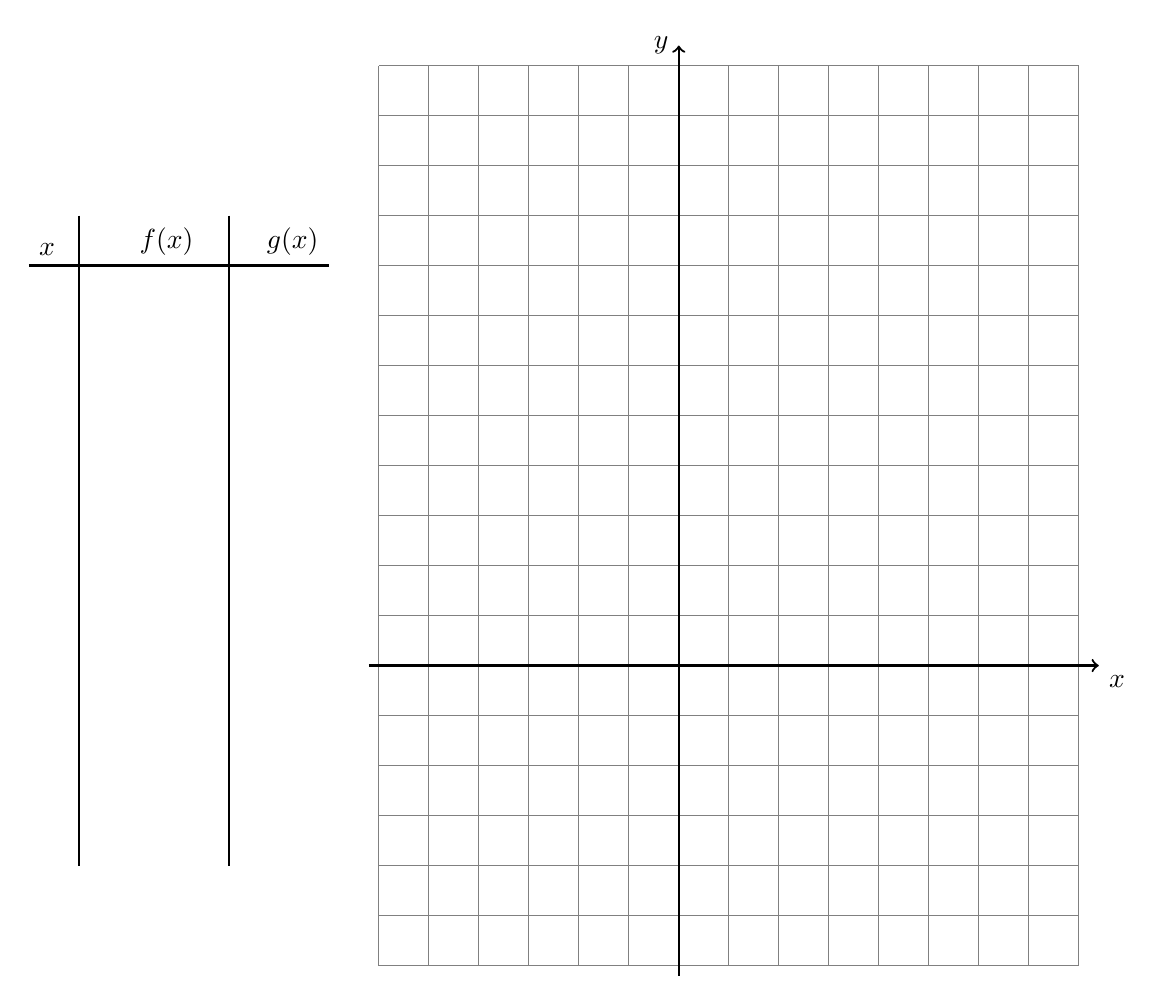
\begin{tikzpicture}[scale=.635]
      \draw [help lines] (-6,-6) grid (8,12);
      \draw [thick, ->] (-6.2,0) -- (8.4,0) node [below right] {$x$};
      \draw [thick, ->] (0,-6.2)--(0,12.4) node [left] {$y$};
      \draw [thick] (-13,8) node[above right]{$x$} --(-9.5,8) node [above left]{$f(x)$}--(-7,8) node [above left]{$g(x)$};
      \draw [thick] (-9,9)--(-9,-4);
      \draw [thick] (-12,9)--(-12,-4);
      \end{tikzpicture}
    \end{center}
    \begin{enumerate}
      \item The parabola is translated two units up, $f \rightarrow g$. \\[0.25cm]
      Draw the parabola $g(x)$ on the graph, marking and labeling its vertex.
      \item Complete the t-chart values for $g(x)$.
      \item What is the equation of $g(x)$? \vspace{2cm}
    \end{enumerate}




\end{enumerate}
\end{document}

\item Complete the t-chart for $x= -2,-1,0,1,2,3,4,5$, then graph and label the function on the grid below, labeling the vertex on the graph as an ordered pair.

  \[h(x) = (x-3)^2\]

    \begin{center} %4 quadrant regents grid w T-Chart
      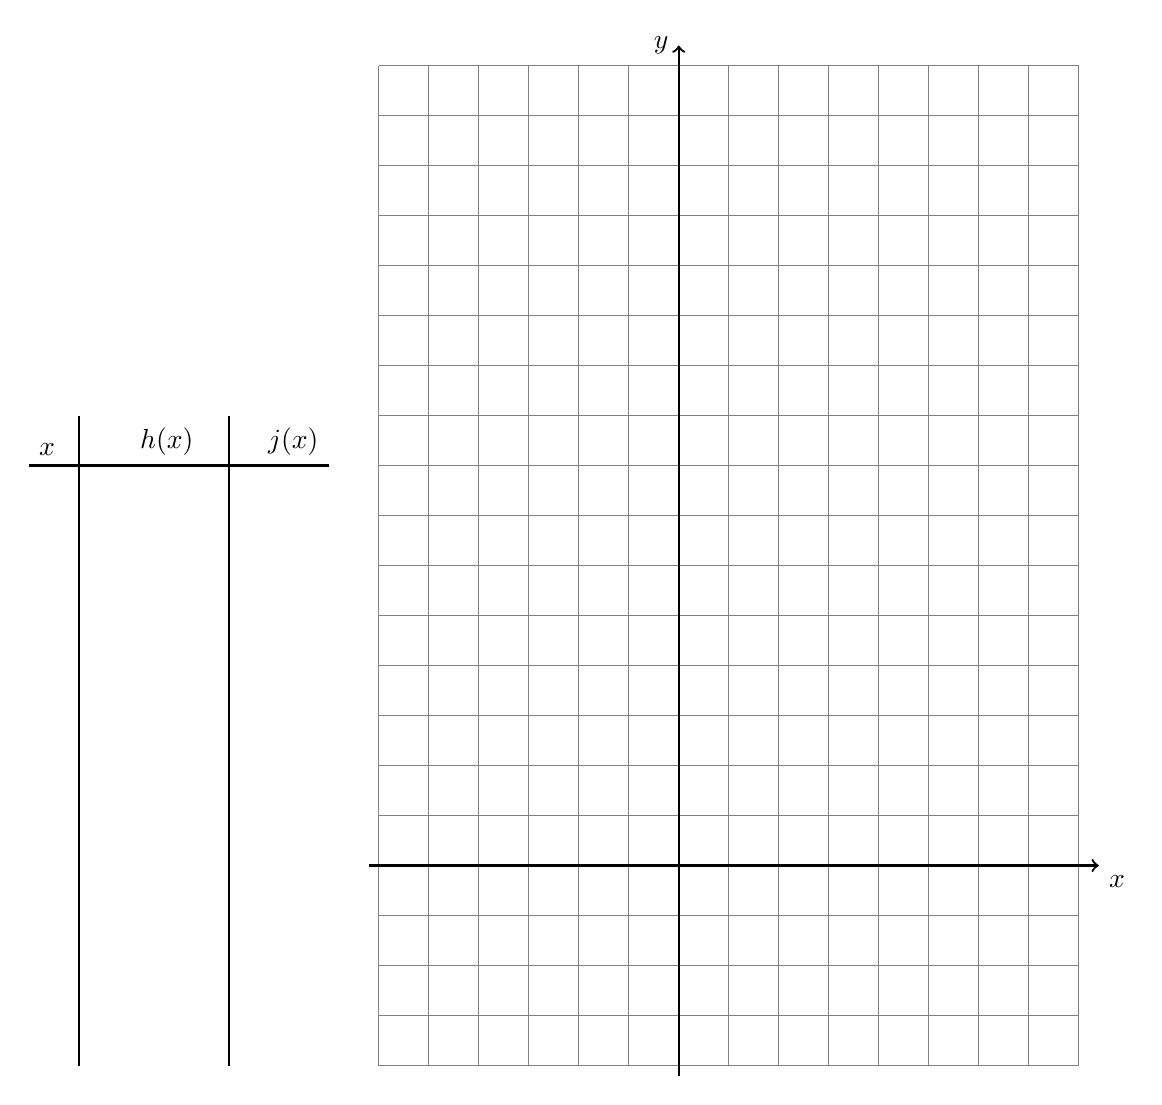
\begin{tikzpicture}[scale=.635]
      \draw [help lines] (-6,-4) grid (8,16);
      \draw [thick, ->] (-6.2,0) -- (8.4,0) node [below right] {$x$};
      \draw [thick, ->] (0,-4.2)--(0,16.4) node [left] {$y$};
      \draw [thick] (-13,8) node[above right]{$x$} --(-9.5,8) node [above left]{$h(x)$}--(-7,8) node [above left]{$j(x)$};
      \draw [thick] (-9,9)--(-9,-4);
      \draw [thick] (-12,9)--(-12,-4);
      \end{tikzpicture}
    \end{center}
    \begin{enumerate}
      \item The parabola is translated three units to the left, $h \rightarrow j$. \\[0.25cm]
      Draw the parabola $j(x)$ on the graph, labeling it and its vertex.
      \item Complete the t-chart values for $j(x)$.
      \item What is the equation of $j(x)$? \vspace{2cm}
    \end{enumerate}